% Options for packages loaded elsewhere
\PassOptionsToPackage{unicode}{hyperref}
\PassOptionsToPackage{hyphens}{url}
%
\documentclass[
  8pt,
  ignorenonframetext,
]{beamer}
\usepackage{pgfpages}
\setbeamertemplate{caption}[numbered]
\setbeamertemplate{caption label separator}{: }
\setbeamercolor{caption name}{fg=normal text.fg}
\beamertemplatenavigationsymbolsempty
% Prevent slide breaks in the middle of a paragraph
\widowpenalties 1 10000
\raggedbottom
\setbeamertemplate{part page}{
  \centering
  \begin{beamercolorbox}[sep=16pt,center]{part title}
    \usebeamerfont{part title}\insertpart\par
  \end{beamercolorbox}
}
\setbeamertemplate{section page}{
  \centering
  \begin{beamercolorbox}[sep=12pt,center]{part title}
    \usebeamerfont{section title}\insertsection\par
  \end{beamercolorbox}
}
\setbeamertemplate{subsection page}{
  \centering
  \begin{beamercolorbox}[sep=8pt,center]{part title}
    \usebeamerfont{subsection title}\insertsubsection\par
  \end{beamercolorbox}
}
\AtBeginPart{
  \frame{\partpage}
}
\AtBeginSection{
  \ifbibliography
  \else
    \frame{\sectionpage}
  \fi
}
\AtBeginSubsection{
  \frame{\subsectionpage}
}

\usepackage{amsmath,amssymb}
\usepackage{iftex}
\ifPDFTeX
  \usepackage[T1]{fontenc}
  \usepackage[utf8]{inputenc}
  \usepackage{textcomp} % provide euro and other symbols
\else % if luatex or xetex
  \usepackage{unicode-math}
  \defaultfontfeatures{Scale=MatchLowercase}
  \defaultfontfeatures[\rmfamily]{Ligatures=TeX,Scale=1}
\fi
\usepackage{lmodern}
\ifPDFTeX\else  
    % xetex/luatex font selection
\fi
% Use upquote if available, for straight quotes in verbatim environments
\IfFileExists{upquote.sty}{\usepackage{upquote}}{}
\IfFileExists{microtype.sty}{% use microtype if available
  \usepackage[]{microtype}
  \UseMicrotypeSet[protrusion]{basicmath} % disable protrusion for tt fonts
}{}
\makeatletter
\@ifundefined{KOMAClassName}{% if non-KOMA class
  \IfFileExists{parskip.sty}{%
    \usepackage{parskip}
  }{% else
    \setlength{\parindent}{0pt}
    \setlength{\parskip}{6pt plus 2pt minus 1pt}}
}{% if KOMA class
  \KOMAoptions{parskip=half}}
\makeatother
\usepackage{xcolor}
\newif\ifbibliography
\setlength{\emergencystretch}{3em} % prevent overfull lines
\setcounter{secnumdepth}{-\maxdimen} % remove section numbering

\usepackage{color}
\usepackage{fancyvrb}
\newcommand{\VerbBar}{|}
\newcommand{\VERB}{\Verb[commandchars=\\\{\}]}
\DefineVerbatimEnvironment{Highlighting}{Verbatim}{commandchars=\\\{\}}
% Add ',fontsize=\small' for more characters per line
\usepackage{framed}
\definecolor{shadecolor}{RGB}{241,243,245}
\newenvironment{Shaded}{\begin{snugshade}}{\end{snugshade}}
\newcommand{\AlertTok}[1]{\textcolor[rgb]{0.68,0.00,0.00}{#1}}
\newcommand{\AnnotationTok}[1]{\textcolor[rgb]{0.37,0.37,0.37}{#1}}
\newcommand{\AttributeTok}[1]{\textcolor[rgb]{0.40,0.45,0.13}{#1}}
\newcommand{\BaseNTok}[1]{\textcolor[rgb]{0.68,0.00,0.00}{#1}}
\newcommand{\BuiltInTok}[1]{\textcolor[rgb]{0.00,0.23,0.31}{#1}}
\newcommand{\CharTok}[1]{\textcolor[rgb]{0.13,0.47,0.30}{#1}}
\newcommand{\CommentTok}[1]{\textcolor[rgb]{0.37,0.37,0.37}{#1}}
\newcommand{\CommentVarTok}[1]{\textcolor[rgb]{0.37,0.37,0.37}{\textit{#1}}}
\newcommand{\ConstantTok}[1]{\textcolor[rgb]{0.56,0.35,0.01}{#1}}
\newcommand{\ControlFlowTok}[1]{\textcolor[rgb]{0.00,0.23,0.31}{#1}}
\newcommand{\DataTypeTok}[1]{\textcolor[rgb]{0.68,0.00,0.00}{#1}}
\newcommand{\DecValTok}[1]{\textcolor[rgb]{0.68,0.00,0.00}{#1}}
\newcommand{\DocumentationTok}[1]{\textcolor[rgb]{0.37,0.37,0.37}{\textit{#1}}}
\newcommand{\ErrorTok}[1]{\textcolor[rgb]{0.68,0.00,0.00}{#1}}
\newcommand{\ExtensionTok}[1]{\textcolor[rgb]{0.00,0.23,0.31}{#1}}
\newcommand{\FloatTok}[1]{\textcolor[rgb]{0.68,0.00,0.00}{#1}}
\newcommand{\FunctionTok}[1]{\textcolor[rgb]{0.28,0.35,0.67}{#1}}
\newcommand{\ImportTok}[1]{\textcolor[rgb]{0.00,0.46,0.62}{#1}}
\newcommand{\InformationTok}[1]{\textcolor[rgb]{0.37,0.37,0.37}{#1}}
\newcommand{\KeywordTok}[1]{\textcolor[rgb]{0.00,0.23,0.31}{#1}}
\newcommand{\NormalTok}[1]{\textcolor[rgb]{0.00,0.23,0.31}{#1}}
\newcommand{\OperatorTok}[1]{\textcolor[rgb]{0.37,0.37,0.37}{#1}}
\newcommand{\OtherTok}[1]{\textcolor[rgb]{0.00,0.23,0.31}{#1}}
\newcommand{\PreprocessorTok}[1]{\textcolor[rgb]{0.68,0.00,0.00}{#1}}
\newcommand{\RegionMarkerTok}[1]{\textcolor[rgb]{0.00,0.23,0.31}{#1}}
\newcommand{\SpecialCharTok}[1]{\textcolor[rgb]{0.37,0.37,0.37}{#1}}
\newcommand{\SpecialStringTok}[1]{\textcolor[rgb]{0.13,0.47,0.30}{#1}}
\newcommand{\StringTok}[1]{\textcolor[rgb]{0.13,0.47,0.30}{#1}}
\newcommand{\VariableTok}[1]{\textcolor[rgb]{0.07,0.07,0.07}{#1}}
\newcommand{\VerbatimStringTok}[1]{\textcolor[rgb]{0.13,0.47,0.30}{#1}}
\newcommand{\WarningTok}[1]{\textcolor[rgb]{0.37,0.37,0.37}{\textit{#1}}}

\providecommand{\tightlist}{%
  \setlength{\itemsep}{0pt}\setlength{\parskip}{0pt}}\usepackage{longtable,booktabs,array}
\usepackage{calc} % for calculating minipage widths
\usepackage{caption}
% Make caption package work with longtable
\makeatletter
\def\fnum@table{\tablename~\thetable}
\makeatother
\usepackage{graphicx}
\makeatletter
\def\maxwidth{\ifdim\Gin@nat@width>\linewidth\linewidth\else\Gin@nat@width\fi}
\def\maxheight{\ifdim\Gin@nat@height>\textheight\textheight\else\Gin@nat@height\fi}
\makeatother
% Scale images if necessary, so that they will not overflow the page
% margins by default, and it is still possible to overwrite the defaults
% using explicit options in \includegraphics[width, height, ...]{}
\setkeys{Gin}{width=\maxwidth,height=\maxheight,keepaspectratio}
% Set default figure placement to htbp
\makeatletter
\def\fps@figure{htbp}
\makeatother

% type setting
% ------------------------------------------------------------------------------
\usepackage[german]{babel}     

% fonts
% ------------------------------------------------------------------------------
\usefonttheme{professionalfonts}

% slide title and horizontal line
% ------------------------------------------------------------------------------
\setbeamertemplate{frametitle}{%
    \vskip-30pt \color{black}\large%
    \begin{minipage}[b][23pt]{120mm}%
    \flushleft\insertframetitle%
    \end{minipage}%
}

\setbeamertemplate{headline}										
{
\vskip10pt\hfill\hspace{3.5mm} 										 
\vskip15pt\color{black}\rule{\textwidth}{0.4pt} 					 
}

% slide number
% ---------------------------------------------------------------
\setbeamertemplate{navigation symbols}{}
\setbeamertemplate{footline}
{
\vskip5pt
\vskip2pt
\makebox[123mm]{\hspace{7.5mm}
\hfill Programmierung und Deskriptive Statistik $\vert$ 
Belinda Fleischmann $\vert$ 
Folie \insertframenumber}
\vskip4pt
}

% block color scheme
% ------------------------------------------------------------------------------
% colors
\definecolor{white}{RGB}{255,255,255}
\definecolor{grey}{RGB}{235,235,235}
\definecolor{middlegrey}{RGB}{210,210,210}
\definecolor{darkgrey}{RGB}{105,105,105}
\definecolor{lightgrey}{RGB}{245,245,245}
\definecolor{linkblue}{HTML}{4F86AB}
\definecolor{darkblue}{RGB}{0,0,139}
\definecolor{darkcyan}{RGB}{5,92,92}
\definecolor{middlecyan}{RGB}{0,153,153}
\definecolor{darkgreen}{RGB}{0,102,51}
\definecolor{plum}{RGB}{128,0,128}


% definitions and theorems
\setbeamercolor{block title}{fg = black, bg = grey}
\setbeamercolor{block body}{fg = black, bg = lightgrey}

% general line spacing 
% ------------------------------------------------------------------------------
\linespread{1.3}

% local line spacing
% ------------------------------------------------------------------------------
\usepackage{setspace}

% colors
% -----------------------------------------------------------------------------
\usepackage{color}
\usepackage{xcolor}

% justified text
% ------------------------------------------------------------------------------
\usepackage{ragged2e}
\usepackage{etoolbox}
\apptocmd{\frame}{}{\justifying}{}

% bullet point lists
% -----------------------------------------------------------------------------
\setbeamertemplate{itemize item}[circle]
\setbeamertemplate{itemize subitem}[circle]
\setbeamertemplate{itemize subsubitem}[circle]
\setbeamercolor{itemize item}{fg = black}
\setbeamercolor{itemize subitem}{fg = black}
\setbeamercolor{itemize subsubitem}{fg = black}
\setbeamercolor{enumerate item}{fg = black}
\setbeamercolor{enumerate subitem}{fg = black}
\setbeamercolor{enumerate subsubitem}{fg = black}
\setbeamerfont{itemize/enumerate body}{}
\setbeamerfont{itemize/enumerate subbody}{size = \normalsize}
\setbeamerfont{itemize/enumerate subsubbody}{size = \normalsize}
\usepackage{pifont} % for different bullet styles

% color links
% ------------------------------------------------------------------------------
\usepackage{hyperref}
\definecolor{urls}{RGB}{204,0,0}
\hypersetup{colorlinks=true, citecolor = urls, urlcolor = urls}

% additional math commands
% ------------------------------------------------------------------------------
\usepackage{bm}                                         % bold math symbols
\newcommand{\niton}{\not\owns}


% additional mathematical operators
% ------------------------------------------------------------------------------
\DeclareMathOperator*{\argmax}{arg\,max}
\DeclareMathOperator*{\argmin}{arg\,min}
\newcommand{\ups}{\upsilon}

% text highlighting
% ------------------------------------------------------------------------------
\usepackage{soul}
\makeatletter
\let\HL\hl
\renewcommand\hl{%
  \let\set@color\beamerorig@set@color
  \let\reset@color\beamerorig@reset@color
  \HL}
\makeatother

% text box colors
\renewcommand\fbox{\fcolorbox{middlegrey}{white}}
\newcommand{\fboxfill}{\fcolorbox{grey}{grey}}

% equation highlighting
% -----------------------------------------------------------------------------
\newcommand{\highlight}[2][yellow]{\mathchoice%
  {\colorbox{#1}{$\displaystyle#2$}}%
  {\colorbox{#1}{$\textstyle#2$}}%
  {\colorbox{#1}{$\scriptstyle#2$}}%
  {\colorbox{#1}{$\scriptscriptstyle#2$}}}%
  
\makeatletter
\makeatother
\makeatletter
\makeatother
\makeatletter
\@ifpackageloaded{caption}{}{\usepackage{caption}}
\AtBeginDocument{%
\ifdefined\contentsname
  \renewcommand*\contentsname{Table of contents}
\else
  \newcommand\contentsname{Table of contents}
\fi
\ifdefined\listfigurename
  \renewcommand*\listfigurename{List of Figures}
\else
  \newcommand\listfigurename{List of Figures}
\fi
\ifdefined\listtablename
  \renewcommand*\listtablename{List of Tables}
\else
  \newcommand\listtablename{List of Tables}
\fi
\ifdefined\figurename
  \renewcommand*\figurename{Figure}
\else
  \newcommand\figurename{Figure}
\fi
\ifdefined\tablename
  \renewcommand*\tablename{Table}
\else
  \newcommand\tablename{Table}
\fi
}
\@ifpackageloaded{float}{}{\usepackage{float}}
\floatstyle{ruled}
\@ifundefined{c@chapter}{\newfloat{codelisting}{h}{lop}}{\newfloat{codelisting}{h}{lop}[chapter]}
\floatname{codelisting}{Listing}
\newcommand*\listoflistings{\listof{codelisting}{List of Listings}}
\makeatother
\makeatletter
\@ifpackageloaded{caption}{}{\usepackage{caption}}
\@ifpackageloaded{subcaption}{}{\usepackage{subcaption}}
\makeatother
\makeatletter
\@ifpackageloaded{tcolorbox}{}{\usepackage[skins,breakable]{tcolorbox}}
\makeatother
\makeatletter
\@ifundefined{shadecolor}{\definecolor{shadecolor}{rgb}{.97, .97, .97}}
\makeatother
\makeatletter
\makeatother
\makeatletter
\makeatother
\ifLuaTeX
  \usepackage{selnolig}  % disable illegal ligatures
\fi
\IfFileExists{bookmark.sty}{\usepackage{bookmark}}{\usepackage{hyperref}}
\IfFileExists{xurl.sty}{\usepackage{xurl}}{} % add URL line breaks if available
\urlstyle{same} % disable monospaced font for URLs
\hypersetup{
  hidelinks,
  pdfcreator={LaTeX via pandoc}}

\author{}
\date{}

\begin{document}
\ifdefined\Shaded\renewenvironment{Shaded}{\begin{tcolorbox}[breakable, boxrule=0pt, sharp corners, borderline west={3pt}{0pt}{shadecolor}, interior hidden, enhanced, frame hidden]}{\end{tcolorbox}}\fi

\begin{frame}[plain]{Titelfolie}
\protect\hypertarget{titelfolie}{}
\center


\includegraphics[width=0.2\textwidth,height=\textheight]{../Abbildungen/otto.png}

\vspace{2mm}

\Large

Programmierung und Deskriptive Statistik \vspace{4mm}

\normalsize

BSc Psychologie WiSe 2023/24

\vspace{15mm}
\normalsize

Belinda Fleischmann

\vspace{3mm}
\scriptsize

Inhalte basieren auf
\href{https://www.ipsy.ovgu.de/ipsy_media/Methodenlehre+I/Wintersemester+2122/Programmierung+und+Deskriptive+Statistik/Vorlesungsfolien.pdf}{Programmierung
und Deskriptive Statistik} von
\href{https://www.ipsy.ovgu.de/Institut/Abteilungen+des+Institutes/Methodenlehre+I+_+Experimentelle+und+Neurowissenschaftliche+Psychologie/Team/Dirk+Ostwald.html}{Dirk
Ostwald}, lizenziert unter
\href{https://creativecommons.org/licenses/by-sa/4.0/deed.de}{CC
BY-NC-SA 4.0}
\end{frame}

\begin{frame}[plain]{Termine}
\protect\hypertarget{termine}{}
\setstretch{1.3}
\vfill
\center
\footnotesize

\renewcommand{\arraystretch}{1.1}
\begin{tabular}{lll}
Datum          & Einheit               & Thema                                  \\\hline
11.10.23       & Einführung            & (1) Einführung \\
18.10.23       & R Grundlagen          & (2) R und Visual Studio Code           \\
25.10.23       & R Grundlagen          & (2) R und Visual Studio Code           \\
\textbf{01.11.23}       & \textbf{R Grundlagen}          & \textbf{(3) Vektoren}\\
08.11.23       & R Grundlagen          & (4) Matrizen                           \\
15.11.23       & R Grundlagen          & (5) Listen und Dataframes              \\
22.11.23       & R Grundlagen          & (6) Datenmanagement                    \\
39.11.23       & R Grundlagen          & (7) Häufigkeitsverteilungen            \\
06.12.23       & R Grundlagen          & (8) Verteilungsfunktionen und Quantile \\
13.12.23       & Deskriptive Statistik & (9) Maße der zentralen Tendenz         \\
20.12.23       & Deskriptive Statistik & (10) Maße der Datenvariabilität        \\
20.12.23       & \textit{Leistungsnachweis Teil 1}        \\
               & \textcolor{gray}{Weihnachtspause}                              \\
10.01.24       & Deskriptive Statistik & (11) Anwendungsbeispiel (Deskriptive Statistik)                   \\
17.01.24       & Inferenzstatistik     & (12) Anwendungsbeispiel (Parameterschätzung, Konfidenzintervalle) \\
24.01.24       & Inferenzstatistik     & (13) Anwendungsbeispiel (Hypothesentest)                          \\
25.01.24       & \textit{Leistungsnachweis Teil 2}                          \\\hline
\end{tabular}
\end{frame}

\begin{frame}[plain]{(3) Vekotren - Titelfolie}
\protect\hypertarget{vekotren---titelfolie}{}
\vfill
\huge
\begin{center}
(3) Vektoren
\end{center}
\vfill
\end{frame}

\begin{frame}[plain]{AGENDA}
\protect\hypertarget{agenda}{}
\large
\setstretch{2.5}
\vfill

Übersicht und Erzeugung

Charakterisierung

Indizierung

Arithmetik

Attribute

Übungen und Selbstkontrollfragen
\end{frame}

\begin{frame}[plain]{Erzeugung ======================================}
\protect\hypertarget{erzeugung}{}
\AtBeginSection{}
\section{Erzeugung}

\large
\setstretch{2.5}
\vfill

\textbf{Übersicht und Erzeugung}

Charakterisierung

Indizierung

Arithmetik

Attribute

Übungen und Selbstkontrollfragen
\end{frame}

\begin{frame}{Übersicht}
\protect\hypertarget{uxfcbersicht}{}
\setstretch{1.5}

\small

\begin{itemize}
\item R operiert mit \textit{Datenstrukturen} (z.B. Vektoren, Matrizen, Listen und Dataframes).
\item Die einfachste dieser Datenstrukturen ist ein Vektor.
\item Vektoren sind geordnete Folgen von Datenwerten, die in \underline{einem} Objekt zusammengefasst sind und \underline{einem} Variablennamen zugewiesen sind.
\item Die einzelnen Datenwerte eines Vektors heißen \textit{Elemente} des Vektors.
\item Vektoren, deren Elemente alle vom gleichen Datentyp sind, heißen \textbf{atomar}.
\item Die zentralen Datentypen sind \textbf{numeric} (\textbf{double}, \textbf{integer}),  \textbf{logical},  \textbf{character}
\end{itemize}

\vspace{1mm}

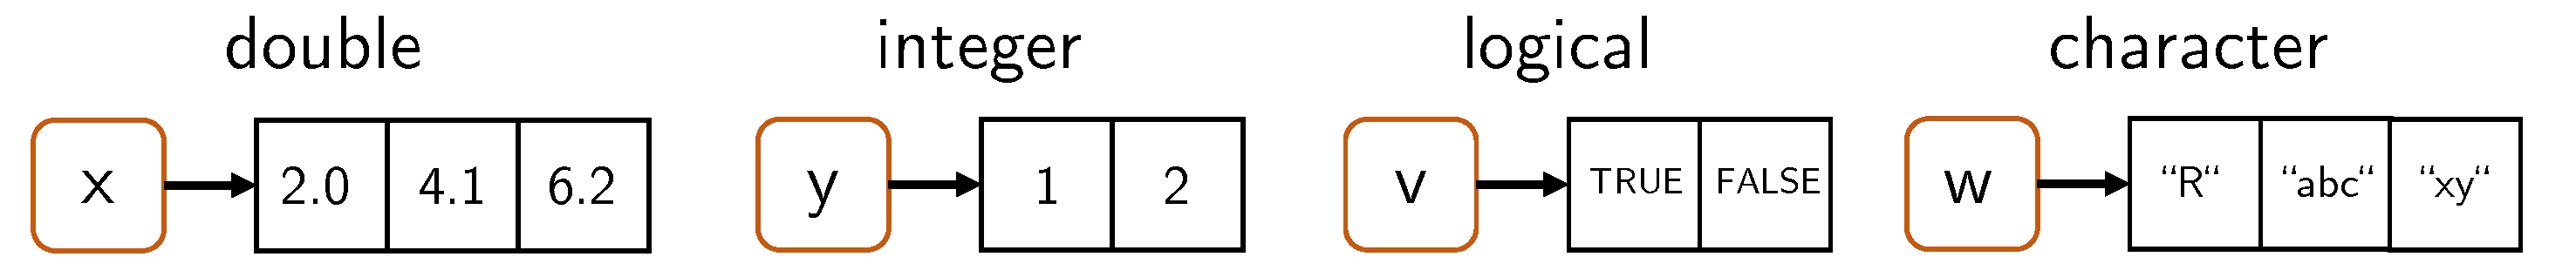
\includegraphics[width=0.9\textwidth,height=\textheight]{../Abbildungen/pds_3_atomic_vectors.pdf}

\begin{itemize}
\tightlist
\item
  Mit dem Begriff \textbf{Vektor} ist hier immer ein \textbf{atomarer
  Vektor} gemeint.
\end{itemize}

\vfill
\end{frame}

\begin{frame}[fragile]{Elementarwerte}
\protect\hypertarget{elementarwerte}{}
\setstretch{1.3}
\small

\textbf{Numeric}

\footnotesize

Per default werden numerische Werte (mit oder ohne Dezimalstellen) als
double initialisiert. Dezimalzahlen können in Dezimalnotation oder
wissenschaftlicher Notation spezifiziert werden. Weitere mögliche Werte
sind Inf, -Inf, und NaN (Not-a-Number). \vspace{1mm} \tiny

\begin{Shaded}
\begin{Highlighting}[]
\NormalTok{h }\OtherTok{\textless{}{-}} \DecValTok{1}                    \CommentTok{\# Einelementiger Vektor vom Typ double (1)}
\NormalTok{i }\OtherTok{\textless{}{-}} \FloatTok{2.1e2}                \CommentTok{\# Einelementiger Vektor vom Typ double (210)}
\NormalTok{j }\OtherTok{\textless{}{-}} \FloatTok{2.1e{-}2}               \CommentTok{\# Einelementiger Vektor vom Typ double (0.021)}
\NormalTok{k }\OtherTok{\textless{}{-}} \ConstantTok{Inf}                  \CommentTok{\# Einelementiger Vektor vom Typ double (unendlich)}
\NormalTok{l }\OtherTok{\textless{}{-}} \ConstantTok{NaN}                  \CommentTok{\# Einelementiger Vektor vom Typ double (NaN)}
\end{Highlighting}
\end{Shaded}

\footnotesize

Integer werden wie double ohne Dezimalstellen spezifiziert, gefolgt von
einem L (long integer). \vspace{1mm} \tiny

\begin{Shaded}
\begin{Highlighting}[]
\NormalTok{x }\OtherTok{\textless{}{-}}\NormalTok{ 1L                   }\CommentTok{\# Einelementiger Vektor vom Typ integer}
\NormalTok{y }\OtherTok{\textless{}{-}}\NormalTok{ 200L                 }\CommentTok{\# Einelementiger Vektor vom Typ integer}
\end{Highlighting}
\end{Shaded}

\small

\textbf{Logical}

\footnotesize

TRUE oder FALSE, abgekürzt T oder F. \vspace{1mm} \tiny

\begin{Shaded}
\begin{Highlighting}[]
\NormalTok{x }\OtherTok{\textless{}{-}} \ConstantTok{TRUE}                 \CommentTok{\# Einelementiger Vektor vom Typ logical}
\NormalTok{y }\OtherTok{\textless{}{-}}\NormalTok{ F                    }\CommentTok{\# Einelementiger Vektor vom Typ logical}
\end{Highlighting}
\end{Shaded}

\small

\textbf{Character}

\footnotesize

Anführungszeichen (``a'') oder Hochkommata (`a'). \vspace{1mm} \tiny

\begin{Shaded}
\begin{Highlighting}[]
\NormalTok{x }\OtherTok{\textless{}{-}} \StringTok{"a"}                  \CommentTok{\# Einelementiger Vektor vom Typ character}
\NormalTok{y }\OtherTok{\textless{}{-}} \StringTok{\textquotesingle{}test\textquotesingle{}}               \CommentTok{\# Einelementiger Vektor vom Typ character}
\end{Highlighting}
\end{Shaded}
\end{frame}

\begin{frame}[fragile]{Erzeugung mehrelementiger Vektoren}
\protect\hypertarget{erzeugung-mehrelementiger-vektoren}{}
\small

Direkte Konkatenation von Elementarwerten mit \texttt{c()}

\tiny

\begin{Shaded}
\begin{Highlighting}[]
\NormalTok{x }\OtherTok{\textless{}{-}} \FunctionTok{c}\NormalTok{(}\DecValTok{1}\NormalTok{, }\DecValTok{2}\NormalTok{, }\DecValTok{3}\NormalTok{)                    }\CommentTok{\# numeric vector [1,2,3]}
\NormalTok{y }\OtherTok{\textless{}{-}} \FunctionTok{c}\NormalTok{(}\DecValTok{0}\NormalTok{, x, }\DecValTok{4}\NormalTok{)                    }\CommentTok{\# numeric vector [0,1,2,3,4]}
\NormalTok{s }\OtherTok{\textless{}{-}} \FunctionTok{c}\NormalTok{(}\StringTok{"a"}\NormalTok{, }\StringTok{"b"}\NormalTok{, }\StringTok{"c"}\NormalTok{)              }\CommentTok{\# character vector ["a", "b", "c"]}
\NormalTok{l }\OtherTok{\textless{}{-}} \FunctionTok{c}\NormalTok{(}\ConstantTok{TRUE}\NormalTok{, }\ConstantTok{FALSE}\NormalTok{)                }\CommentTok{\# logical  vector [TRUE, FALSE]}
\end{Highlighting}
\end{Shaded}

\begin{itemize}
\item
  \footnotesize Beachte: \texttt{c()} konkateniert die Eingabeargumente
  und erzwingt einen einheitlichen Datentyp (vgl. coercion) \tiny

\begin{Shaded}
\begin{Highlighting}[]
\NormalTok{x }\OtherTok{\textless{}{-}} \FunctionTok{c}\NormalTok{(}\DecValTok{1}\NormalTok{, }\StringTok{"a"}\NormalTok{, }\ConstantTok{TRUE}\NormalTok{)         }\CommentTok{\# character vector ["1", "a", "TRUE"]}
\end{Highlighting}
\end{Shaded}
\end{itemize}

\small

Erzeugen ``leerer'' Vektoren mit \texttt{vector()}

\tiny

\begin{Shaded}
\begin{Highlighting}[]
\NormalTok{v }\OtherTok{\textless{}{-}} \FunctionTok{vector}\NormalTok{(}\StringTok{"double"}\NormalTok{, }\DecValTok{3}\NormalTok{)           }\CommentTok{\# double vector [0,0,0]}
\NormalTok{w }\OtherTok{\textless{}{-}} \FunctionTok{vector}\NormalTok{(}\StringTok{"integer"}\NormalTok{, }\DecValTok{3}\NormalTok{)          }\CommentTok{\# integer vector [0,0,0]}
\NormalTok{l }\OtherTok{\textless{}{-}} \FunctionTok{vector}\NormalTok{(}\StringTok{"logical"}\NormalTok{, }\DecValTok{2}\NormalTok{)          }\CommentTok{\# logical vector [FALSE, FALSE]}
\NormalTok{s }\OtherTok{\textless{}{-}} \FunctionTok{vector}\NormalTok{(}\StringTok{"character"}\NormalTok{, }\DecValTok{4}\NormalTok{)        }\CommentTok{\# character vector ["", "", "", ""]}
\end{Highlighting}
\end{Shaded}

\small

Erzeugen ``leerer'' Vektoren mit double(), integer(), logical(),
character()

\tiny

\begin{Shaded}
\begin{Highlighting}[]
\NormalTok{v }\OtherTok{\textless{}{-}} \FunctionTok{double}\NormalTok{(}\DecValTok{3}\NormalTok{)                     }\CommentTok{\# double vector [0,0,0]}
\NormalTok{w }\OtherTok{\textless{}{-}} \FunctionTok{integer}\NormalTok{(}\DecValTok{3}\NormalTok{)                    }\CommentTok{\# integer vector [0,0,0]}
\NormalTok{l }\OtherTok{\textless{}{-}} \FunctionTok{logical}\NormalTok{(}\DecValTok{2}\NormalTok{)                    }\CommentTok{\# logical vector [FALSE, FALSE]}
\NormalTok{s }\OtherTok{\textless{}{-}} \FunctionTok{character}\NormalTok{(}\DecValTok{4}\NormalTok{)                  }\CommentTok{\# character vector ["", "", "", ""]}
\end{Highlighting}
\end{Shaded}
\end{frame}

\begin{frame}[fragile]{Erzeugung von Vektoren als Sequenzen}
\protect\hypertarget{erzeugung-von-vektoren-als-sequenzen}{}
\small

Erzeugen von ganzzahligen Sequenzen mithilfe des \textbf{Colonoperators}
\texttt{:}

\texttt{a:b} erzeugt ganzzahlige Sequenzen von a (inklusive) bis b
(maximal)

\tiny

\begin{Shaded}
\begin{Highlighting}[]
\NormalTok{x }\OtherTok{\textless{}{-}} \DecValTok{0}\SpecialCharTok{:}\DecValTok{5}                         \CommentTok{\# [0,1,2,3,4,5]}
\NormalTok{y }\OtherTok{\textless{}{-}} \FloatTok{1.5}\SpecialCharTok{:}\FloatTok{6.1}                     \CommentTok{\# [1.5, 2.5, 3.5, 4.5, 5.5]}
\end{Highlighting}
\end{Shaded}

\small

Erzeugen von Sequenzen mit \texttt{seq()}

\texttt{seq(from,\ to,\ by\ =\ ((to\ -\ from)/(len\ -\ 1),\ len\ =\ NULL,\ ...)}

\tiny

\begin{Shaded}
\begin{Highlighting}[]
\NormalTok{x\_1 }\OtherTok{\textless{}{-}} \FunctionTok{seq}\NormalTok{(}\DecValTok{0}\NormalTok{, }\DecValTok{5}\NormalTok{)                 }\CommentTok{\# wie 0:5, [0,1,2,3,4,5]}
\NormalTok{x\_2 }\OtherTok{\textless{}{-}} \FunctionTok{seq}\NormalTok{(}\DecValTok{0}\NormalTok{, }\DecValTok{1}\NormalTok{, }\AttributeTok{len =} \DecValTok{5}\NormalTok{)        }\CommentTok{\# 5 Zahlen zwischen 0 (inkl.) und 1 (inkl.), equidistant}
                                 \CommentTok{\# [0.00, 0.25, 0.50, 0.75, 1.00]}
\NormalTok{x\_3 }\OtherTok{\textless{}{-}} \FunctionTok{seq}\NormalTok{(}\DecValTok{0}\NormalTok{, }\DecValTok{2}\NormalTok{, }\AttributeTok{by =}\NormalTok{ .}\DecValTok{15}\NormalTok{)       }\CommentTok{\# 0.15 Schritte zwischen 0 (inkl.) und 2 (max.)}
                                 \CommentTok{\# [0.00, 0.15, 0.30, ..., 1.50 1.65 1.80 1.95]}
\NormalTok{x\_4 }\OtherTok{\textless{}{-}} \FunctionTok{seq}\NormalTok{(}\DecValTok{1}\NormalTok{, }\DecValTok{0}\NormalTok{, }\AttributeTok{by =} \SpecialCharTok{{-}}\NormalTok{.}\DecValTok{1}\NormalTok{)       }\CommentTok{\# {-}0.1 Schritte zwischen 1 (inkl.) und 0 (min.)}
                                 \CommentTok{\# [1.0 0.9 0.8 0.7 0.6 0.5 0.4 0.3 0.2 0.1 0.0]}
\end{Highlighting}
\end{Shaded}

\small

\texttt{seq.int()}, \texttt{seq\_len()}, \texttt{seq\_along()} als
weitere Varianten

\tiny

\begin{Shaded}
\begin{Highlighting}[]
\NormalTok{x\_1 }\OtherTok{\textless{}{-}} \FunctionTok{seq.int}\NormalTok{(}\DecValTok{0}\NormalTok{, }\DecValTok{5}\NormalTok{)             }\CommentTok{\# wie 0:5, [0,1,2,3,4,5]}
\NormalTok{x\_2 }\OtherTok{\textless{}{-}} \FunctionTok{seq\_len}\NormalTok{(}\DecValTok{5}\NormalTok{)                }\CommentTok{\# Natuerliche Zahlen bis 5, [1,2,3,4,5]}
\NormalTok{x\_3 }\OtherTok{\textless{}{-}} \FunctionTok{seq\_along}\NormalTok{(}\FunctionTok{c}\NormalTok{(}\StringTok{"a"}\NormalTok{, }\StringTok{"b"}\NormalTok{))    }\CommentTok{\# wie seq\_len(length(c("a", "b")))}
\end{Highlighting}
\end{Shaded}
\end{frame}

\begin{frame}[plain]{Charakterisierung
======================================}
\protect\hypertarget{charakterisierung}{}
\AtBeginSection{}
\section{Charakterisierung}

\large
\setstretch{2.5}
\vfill

Übersicht und Erzeugung

\textbf{Charakterisierung}

Indizierung

Arithmetik

Attribute

Übungen und Selbstkontrollfragen
\end{frame}

\begin{frame}[fragile]{Vektoreigenschaften ausgeben}
\protect\hypertarget{vektoreigenschaften-ausgeben}{}
\setstretch{0.9}
\small

\texttt{length()} gibt die Anzahl der Elemente eines Vektors aus \tiny

\begin{Shaded}
\begin{Highlighting}[]
\NormalTok{x }\OtherTok{\textless{}{-}} \DecValTok{0}\SpecialCharTok{:}\DecValTok{10}          \CommentTok{\# Vektor}
\FunctionTok{length}\NormalTok{(x)          }\CommentTok{\# Anzahl der Elemente des Vektors}
\end{Highlighting}
\end{Shaded}

\begin{verbatim}
[1] 11
\end{verbatim}

\vspace{2mm}
\small

\texttt{typeof()} gibt den elementaren Datentyp eines Vektors aus

\tiny

\begin{Shaded}
\begin{Highlighting}[]
\NormalTok{x }\OtherTok{\textless{}{-}} \DecValTok{1}\SpecialCharTok{:}\NormalTok{3L          }\CommentTok{\# Vektor}
\FunctionTok{typeof}\NormalTok{(x)          }\CommentTok{\# Datentyp des atomic vectors}
\end{Highlighting}
\end{Shaded}

\begin{verbatim}
[1] "integer"
\end{verbatim}

\vspace{2mm}

\begin{Shaded}
\begin{Highlighting}[]
\NormalTok{y }\OtherTok{\textless{}{-}} \FunctionTok{c}\NormalTok{(T,F,T)      }\CommentTok{\# Vektor}
\FunctionTok{typeof}\NormalTok{(y)          }\CommentTok{\# Der Datentyp des atomic vectors}
\end{Highlighting}
\end{Shaded}

\begin{verbatim}
[1] "logical"
\end{verbatim}

\vspace{2mm}

\indent Anmerkung: \texttt{mode()} und \texttt{storage.mode()} werden
nicht empfohlen, sie existieren für S Kompatibilität.

\vspace{3mm}
\small

\texttt{is.logical()}, \texttt{is.double()}, \texttt{is.integer()},
\texttt{is.character()} testen den Datentyp

\tiny

\begin{Shaded}
\begin{Highlighting}[]
\FunctionTok{is.double}\NormalTok{(x)       }\CommentTok{\# Testen, ob der x vom Typ double ist}
\end{Highlighting}
\end{Shaded}

\begin{verbatim}
[1] FALSE
\end{verbatim}

\vspace{2mm}

\begin{Shaded}
\begin{Highlighting}[]
\FunctionTok{is.logical}\NormalTok{(y)      }\CommentTok{\# Testen, ob der y vom Typ logical ist}
\end{Highlighting}
\end{Shaded}

\begin{verbatim}
[1] TRUE
\end{verbatim}
\end{frame}

\begin{frame}[fragile]{Datentypangleichung (Coercion)}
\protect\hypertarget{datentypangleichung-coercion}{}
\vspace{2mm}
\setstretch{0.9}

\small

Bei Konkatenation verschiedener Datentypen wird ein einheitlicher
Datentyp erzwungen. Es gilt

\center

character \(>\) double \(>\) integer \(>\) logical \vspace{2mm}

\justifying
\footnotesize
\vspace{3mm}

\begin{Shaded}
\begin{Highlighting}[]
\NormalTok{x }\OtherTok{\textless{}{-}} \FunctionTok{c}\NormalTok{(}\FloatTok{1.2}\NormalTok{, }\StringTok{"a"}\NormalTok{)     }\CommentTok{\# Kombination gemischter Datentypen (character schlaegt double)}
\NormalTok{x}
\end{Highlighting}
\end{Shaded}

\begin{verbatim}
[1] "1.2" "a"  
\end{verbatim}

\begin{Shaded}
\begin{Highlighting}[]
\FunctionTok{typeof}\NormalTok{(x)            }\CommentTok{\# Erzeugter Vektor ist vom Datentyp character}
\end{Highlighting}
\end{Shaded}

\begin{verbatim}
[1] "character"
\end{verbatim}

\vspace{2mm}

\begin{Shaded}
\begin{Highlighting}[]
\NormalTok{y }\OtherTok{\textless{}{-}} \FunctionTok{c}\NormalTok{(1L, }\ConstantTok{TRUE}\NormalTok{)     }\CommentTok{\# Kombination  gemischter Datentypen (integer schlaegt logical)}
\NormalTok{y}
\end{Highlighting}
\end{Shaded}

\begin{verbatim}
[1] 1 1
\end{verbatim}

\begin{Shaded}
\begin{Highlighting}[]
\FunctionTok{typeof}\NormalTok{(y)            }\CommentTok{\# Erzeugter Vektor ist vom Typ integer}
\end{Highlighting}
\end{Shaded}

\begin{verbatim}
[1] "integer"
\end{verbatim}

\vfill
\end{frame}

\begin{frame}[fragile]{Datentypangleichung (Coercion)}
\protect\hypertarget{datentypangleichung-coercion-1}{}
\vspace{2mm}
\setstretch{1.2}

\justifying
\small

Explizite Coercion mit \texttt{as.logical()}, \texttt{as.integer()},
\texttt{as.double()}, \texttt{as.character()} \vspace{1mm}

\footnotesize

\begin{Shaded}
\begin{Highlighting}[]
\NormalTok{x }\OtherTok{\textless{}{-}} \FunctionTok{c}\NormalTok{(}\DecValTok{0}\NormalTok{, }\DecValTok{1}\NormalTok{, }\DecValTok{1}\NormalTok{, }\DecValTok{0}\NormalTok{)        }\CommentTok{\# double Vektor}
\NormalTok{y }\OtherTok{\textless{}{-}} \FunctionTok{as.logical}\NormalTok{(x)        }\CommentTok{\# ... umgewandelt in logical}
\NormalTok{y}
\end{Highlighting}
\end{Shaded}

\begin{verbatim}
[1] FALSE  TRUE  TRUE FALSE
\end{verbatim}

\vspace{3mm}
\small

Coercion geschieht aber auch oft implizit: \vspace{1mm}

\footnotesize

\begin{Shaded}
\begin{Highlighting}[]
\NormalTok{x }\OtherTok{\textless{}{-}} \FunctionTok{c}\NormalTok{(T, F, T, T)        }\CommentTok{\# logical Vektor}
\NormalTok{s }\OtherTok{\textless{}{-}} \FunctionTok{sum}\NormalTok{(x)               }\CommentTok{\# Summation in integer gewandelter logical Elemente}
\NormalTok{s}
\end{Highlighting}
\end{Shaded}

\begin{verbatim}
[1] 3
\end{verbatim}

\vfill
\end{frame}

\begin{frame}[plain]{Indizierung ======================================}
\protect\hypertarget{indizierung}{}
\AtBeginSection{}
\section{Indizierung}

\large
\setstretch{2.5}
\vfill

Übersicht und Erzeugung

Charakterisierung

\textbf{Indizierung}

Arithmetik

Attribute

Übungen und Selbstkontrollfragen
\end{frame}

\begin{frame}[fragile]{Indizierung}
\protect\hypertarget{indizierung-1}{}
\setstretch{1.5}

\normalsize

\textcolor{darkblue}{Grundlagen} \vspace{-2mm}

\small

\begin{itemize}
\tightlist
\item
  Einzelne oder mehrere Vektorkomponenten werden durch Indizierung
  adressiert.
\item
  Indizierung wird auch Indexing, Subsetting, oder Slicing genannt.
\item
  Zur Indizierung werden eckige Klammern {[}\(\,\,\){]} benutzt.
\item
  Indizierung kann zur Kopie oder Manipulation von Komponenten benutzt
  werden.
\item
  Der Index des ersten Elements ist 1 (nicht 0, wie in anderen
  Sprachen).
\end{itemize}

\vspace{1mm}
\normalsize

\textcolor{darkcyan}{Beispiel} \tiny

\begin{Shaded}
\begin{Highlighting}[]
\NormalTok{x }\OtherTok{\textless{}{-}} \FunctionTok{c}\NormalTok{(}\StringTok{"a"}\NormalTok{, }\StringTok{"b"}\NormalTok{, }\StringTok{"c"}\NormalTok{)   }\CommentTok{\# character vector ["a", "b", "c"]}
\NormalTok{y }\OtherTok{\textless{}{-}}\NormalTok{ x[}\DecValTok{2}\NormalTok{]               }\CommentTok{\# Kopie von "b" in y}
\NormalTok{x[}\DecValTok{3}\NormalTok{] }\OtherTok{\textless{}{-}} \StringTok{"d"}             \CommentTok{\# Aenderung von x zu x = ["a", "b", "d"]}
\end{Highlighting}
\end{Shaded}

\vspace{1mm}
\normalsize

\textcolor{darkblue}{Prinzipien der Indizierung in R}

\small

\begin{itemize}
\tightlist
\item
  Ein \textbf{Vektor positiver Zahlen} adressiert entsprechende
  Komponenten.
\item
  Ein \textbf{Vektor negativer Zahlen} adressiert komplementäre
  Komponenten.
\item
  Ein \textbf{logischen Vektor} adressiert die Komponenten mit TRUE.
\item
  Ein \textbf{character Vektor} adressiert benannte Komponenten.
\end{itemize}
\end{frame}

\begin{frame}[fragile]{\textcolor{darkcyan}{Beispiele}}
\protect\hypertarget{section}{}
\footnotesize

Indizierung mit einem \textbf{Vektor positiver Zahlen}

\begin{Shaded}
\begin{Highlighting}[]
\NormalTok{x }\OtherTok{\textless{}{-}} \FunctionTok{c}\NormalTok{(}\DecValTok{1}\NormalTok{ ,}\DecValTok{4}\NormalTok{ ,}\DecValTok{9}\NormalTok{ ,}\DecValTok{16}\NormalTok{ ,}\DecValTok{25}\NormalTok{)   }\CommentTok{\# [1,4,9,16,25] = [1\^{}2, 2\^{}2, 3\^{}2, 4\^{}2, 5\^{}2]}
\NormalTok{y }\OtherTok{\textless{}{-}}\NormalTok{ x[}\DecValTok{1}\SpecialCharTok{:}\DecValTok{3}\NormalTok{]               }\CommentTok{\# 1:3 erzeugt Vektor [1,2,3], x[1:3] = x[c(1,2,3)] = [1,4,9]}
\NormalTok{z }\OtherTok{\textless{}{-}}\NormalTok{ x[}\FunctionTok{c}\NormalTok{(}\DecValTok{1}\NormalTok{, }\DecValTok{3}\NormalTok{, }\DecValTok{5}\NormalTok{)]        }\CommentTok{\# c(1,3,5) erzeugt Vektor [1,3,5], x[c(1,3,5)] = [1,9,25]}
\end{Highlighting}
\end{Shaded}

Indizierung mit einem \textbf{Vektor negativer Zahlen}

\begin{Shaded}
\begin{Highlighting}[]
\NormalTok{x }\OtherTok{\textless{}{-}} \FunctionTok{c}\NormalTok{(}\DecValTok{1}\NormalTok{, }\DecValTok{4}\NormalTok{, }\DecValTok{9}\NormalTok{, }\DecValTok{16}\NormalTok{, }\DecValTok{25}\NormalTok{)   }\CommentTok{\# [1,4,9,16,25] = [1\^{}2, 2\^{}2, 3\^{}2, 4\^{}2, 5\^{}2]}
\NormalTok{y }\OtherTok{\textless{}{-}}\NormalTok{ x[}\FunctionTok{c}\NormalTok{(}\SpecialCharTok{{-}}\DecValTok{2}\NormalTok{, }\SpecialCharTok{{-}}\DecValTok{4}\NormalTok{)]         }\CommentTok{\# Alle Komponenten ausser 2 und 4, x[c({-}2,{-}4)] = [1,9,25]}
\NormalTok{z }\OtherTok{\textless{}{-}}\NormalTok{ x[}\FunctionTok{c}\NormalTok{(}\SpecialCharTok{{-}}\DecValTok{1}\NormalTok{, }\DecValTok{2}\NormalTok{)]          }\CommentTok{\# Gemischte Indizierung nicht erlaubt (Fehlermeldung)}
\end{Highlighting}
\end{Shaded}

Indizierung mit einem \textbf{logischen Vektor}

\begin{Shaded}
\begin{Highlighting}[]
\NormalTok{x }\OtherTok{\textless{}{-}} \FunctionTok{c}\NormalTok{(}\DecValTok{1}\NormalTok{, }\DecValTok{4}\NormalTok{, }\DecValTok{9}\NormalTok{, }\DecValTok{16}\NormalTok{ ,}\DecValTok{25}\NormalTok{)   }\CommentTok{\# [1,4,9,16,25] = [1\^{}2, 2\^{}2, 3\^{}2, 4\^{}2, 5\^{}2]}
\NormalTok{y }\OtherTok{\textless{}{-}}\NormalTok{ x[}\FunctionTok{c}\NormalTok{(T, T, F, F, T)]  }\CommentTok{\# TRUE Komponenten,  x[c(T,T,F,F,T)] = [1,4,25]}
\NormalTok{z }\OtherTok{\textless{}{-}}\NormalTok{ x[x }\SpecialCharTok{\textgreater{}} \DecValTok{5}\NormalTok{]             }\CommentTok{\# x \textgreater{} 5 = [F,F,T,T,T], x[x \textgreater{} 5] = [9,16,25]}
\end{Highlighting}
\end{Shaded}

Indizierung mit einem \textbf{character Vektor}

\begin{Shaded}
\begin{Highlighting}[]
\NormalTok{x }\OtherTok{\textless{}{-}} \FunctionTok{c}\NormalTok{(}\DecValTok{1}\NormalTok{, }\DecValTok{4}\NormalTok{, }\DecValTok{9}\NormalTok{, }\DecValTok{16}\NormalTok{, }\DecValTok{25}\NormalTok{)   }\CommentTok{\# [1,4,9,16,25] = [1\^{}2, 2\^{}2, 3\^{}2, 4\^{}2, 5\^{}2]}
\FunctionTok{names}\NormalTok{(x) }\OtherTok{\textless{}{-}} \FunctionTok{c}\NormalTok{(}\StringTok{"a"}\NormalTok{,}\StringTok{"b"}\NormalTok{)    }\CommentTok{\# Benennung der Komponenten als [a  b \textless{}NA\textgreater{} \textless{}NA\textgreater{} \textless{}NA\textgreater{}]}
\NormalTok{y }\OtherTok{\textless{}{-}}\NormalTok{ x[}\StringTok{"a"}\NormalTok{]               }\CommentTok{\# x["a"] = 1}
\end{Highlighting}
\end{Shaded}
\end{frame}

\begin{frame}[fragile]{Anmerkungen zur Indizierung in R}
\protect\hypertarget{anmerkungen-zur-indizierung-in-r}{}
\normalsize

R hat eine (zu) hohe Flexibilität bei Indizierung

\small
\vspace{1mm}

Out-of-range Indizes verursachen keine Fehler, sondern geben NA aus
\footnotesize

\begin{Shaded}
\begin{Highlighting}[]
\NormalTok{x }\OtherTok{\textless{}{-}} \FunctionTok{c}\NormalTok{(}\DecValTok{1}\NormalTok{, }\DecValTok{4}\NormalTok{, }\DecValTok{9}\NormalTok{, }\DecValTok{16}\NormalTok{, }\DecValTok{25}\NormalTok{)  }\CommentTok{\# [1,4,9,16,25] = [1\^{}2, 2\^{}2, 3\^{}2, 4\^{}2, 5\^{}2]}
\NormalTok{y }\OtherTok{\textless{}{-}}\NormalTok{ x[}\DecValTok{10}\NormalTok{]               }\CommentTok{\# x[10] = NA (Not Applicable)}
\end{Highlighting}
\end{Shaded}

\vspace{1mm}

Nichtganzzahlige Indizes verursachen keine Fehler, sondern werden
abgerundet \footnotesize

\begin{Shaded}
\begin{Highlighting}[]
\NormalTok{y }\OtherTok{\textless{}{-}}\NormalTok{ x[}\FloatTok{4.9}\NormalTok{]              }\CommentTok{\# x[4.9] = x[4] = 16}
\NormalTok{z }\OtherTok{\textless{}{-}}\NormalTok{ x[}\SpecialCharTok{{-}}\FloatTok{4.9}\NormalTok{]             }\CommentTok{\# x[{-}4.9] = x[{-}4] = [1,4,9,25]}
\end{Highlighting}
\end{Shaded}

\vspace{1mm}

Leere Indizes indizieren den gesamten Vektor \footnotesize

\begin{Shaded}
\begin{Highlighting}[]
\NormalTok{y }\OtherTok{\textless{}{-}}\NormalTok{ x[]                 }\CommentTok{\# y = x}
\end{Highlighting}
\end{Shaded}

\vfill
\end{frame}

\begin{frame}[plain]{Arithmetik ======================================}
\protect\hypertarget{arithmetik}{}
\AtBeginSection{}
\section{Arithmetik}

\large
\setstretch{2.5}
\vfill

Übersicht und Erzeugung

Charakterisierung

Indizierung

\textbf{Arithmetik}

Attribute

Übungen und Selbstkontrollfragen
\end{frame}

\begin{frame}[fragile]{Elementweise Auswertung}
\protect\hypertarget{elementweise-auswertung}{}
\small

\textbf{\textcolor{darkblue}{Unitäre}} arithmetische Operatoren und
Funktionen werden elementweise ausgewertet

\footnotesize

\begin{Shaded}
\begin{Highlighting}[]
\NormalTok{a }\OtherTok{\textless{}{-}} \FunctionTok{seq}\NormalTok{(}\DecValTok{0}\NormalTok{, }\DecValTok{1}\NormalTok{, }\AttributeTok{len =} \DecValTok{11}\NormalTok{) }\CommentTok{\# a = [ 0.0, 0.1 , ..., 0.9, 1.0]}
\NormalTok{b }\OtherTok{\textless{}{-}} \SpecialCharTok{{-}}\NormalTok{a                  }\CommentTok{\# b = [{-}0.0, {-}0.1, ..., {-}0.9, {-}1.0]}
\NormalTok{v }\OtherTok{\textless{}{-}}\NormalTok{ a}\SpecialCharTok{\^{}}\DecValTok{2}                 \CommentTok{\# v = [ 0.0\^{}2 ,  0.1\^{}2 , ..., 0.9\^{}2, 1.0\^{}2]}
\NormalTok{w }\OtherTok{\textless{}{-}} \FunctionTok{log}\NormalTok{(a)              }\CommentTok{\# w = [ln(0.0), ln(0.1), ..., ln(0.9), ln(1.0)]}
\end{Highlighting}
\end{Shaded}

\small

\textbf{\textcolor{darkblue}{Binäre}} arithmetische Operatoren werden
elementweise ausgewertet

\footnotesize

Vektoren gleicher Länge

\begin{Shaded}
\begin{Highlighting}[]
\NormalTok{a }\OtherTok{\textless{}{-}} \FunctionTok{c}\NormalTok{(}\DecValTok{1}\NormalTok{, }\DecValTok{2}\NormalTok{, }\DecValTok{3}\NormalTok{)          }\CommentTok{\# a = [1,2,3]}
\NormalTok{b }\OtherTok{\textless{}{-}} \FunctionTok{c}\NormalTok{(}\DecValTok{2}\NormalTok{, }\DecValTok{1}\NormalTok{, }\DecValTok{4}\NormalTok{)          }\CommentTok{\# b = [2,1,4]}
\NormalTok{v }\OtherTok{\textless{}{-}}\NormalTok{ a }\SpecialCharTok{+}\NormalTok{ b               }\CommentTok{\# v = [1,2,3] + [2,1,4] = [1+2,2+1,3+4] = [3,3,7]}
\NormalTok{w }\OtherTok{\textless{}{-}}\NormalTok{ a }\SpecialCharTok{{-}}\NormalTok{ b               }\CommentTok{\# w = [1,2,3] {-} [2,1,4] = [1{-}2,2{-}1,3{-}4] = [{-}1, 1, {-}1]}
\NormalTok{x }\OtherTok{\textless{}{-}}\NormalTok{ a }\SpecialCharTok{*}\NormalTok{ b               }\CommentTok{\# x = [1,2,3] * [2,1,4] = [1*2,2*1,3*4] = [2, 2, 12]}
\NormalTok{y }\OtherTok{\textless{}{-}}\NormalTok{ a }\SpecialCharTok{/}\NormalTok{ b               }\CommentTok{\# y = [1,2,3] / [2,1,4] = [1/2,2/1,3/4] = [0.50, 2, 0.75]}
\end{Highlighting}
\end{Shaded}

\footnotesize

Vektoren und Skalare (= Vektoren der Länge 1)

\begin{Shaded}
\begin{Highlighting}[]
\NormalTok{a }\OtherTok{\textless{}{-}} \FunctionTok{c}\NormalTok{(}\DecValTok{1}\NormalTok{, }\DecValTok{2}\NormalTok{, }\DecValTok{3}\NormalTok{)        }\CommentTok{\# a = [1,2,3]}
\NormalTok{b }\OtherTok{\textless{}{-}} \DecValTok{2}                 \CommentTok{\# b = [2]}
\NormalTok{v }\OtherTok{\textless{}{-}}\NormalTok{ a }\SpecialCharTok{+}\NormalTok{ b             }\CommentTok{\# v = [1,2,3] + [2,2,2] = [1+2,2+2,3+2] = [3, 4, 5]}
\NormalTok{w }\OtherTok{\textless{}{-}}\NormalTok{ a }\SpecialCharTok{{-}}\NormalTok{ b             }\CommentTok{\# w = [1,2,3] {-} [2,2,2] = [1{-}2,2{-}2,3{-}2] = [{-}1, 2, 1]}
\NormalTok{x }\OtherTok{\textless{}{-}}\NormalTok{ a }\SpecialCharTok{*}\NormalTok{ b             }\CommentTok{\# x = [1,2,3] * [2,2,2] = [1*2,2*2,3*2] = [2, 4, 6]}
\NormalTok{y }\OtherTok{\textless{}{-}}\NormalTok{ a }\SpecialCharTok{/}\NormalTok{ b             }\CommentTok{\# y = [1,2,3] / [2,2,2] = [1/2,2/2,3/2] = [0.5, 1, 1.5]}
\end{Highlighting}
\end{Shaded}
\end{frame}

\begin{frame}[fragile]{Recycling}
\protect\hypertarget{recycling}{}
\small
\setstretch{1.4}

\begin{itemize}
\item
  R erlaubt (leider) auch Arithmetik mit Vektoren unterschiedlicher
  Länge
\item
  Bei ganzzahligen Vielfachen der Länge wird der kürzere Vektor
  wiederholt. \footnotesize

\begin{Shaded}
\begin{Highlighting}[]
\NormalTok{x }\OtherTok{\textless{}{-}} \DecValTok{1}\SpecialCharTok{:}\DecValTok{2}                \CommentTok{\# x = [1,2], length(x) = 2}
\NormalTok{y }\OtherTok{\textless{}{-}} \DecValTok{3}\SpecialCharTok{:}\DecValTok{6}                \CommentTok{\# y = [3,4,5,6], length(y) = 4}
\NormalTok{v }\OtherTok{\textless{}{-}}\NormalTok{ x }\SpecialCharTok{+}\NormalTok{ y              }\CommentTok{\# v = [1,2,1,2] + [3,4,5,6] = [4,6,6,8]}
\end{Highlighting}
\end{Shaded}
\item
  \small Arithmetik von Vektoren und Skalaren ist ein Spezialfall dieses
  Prinzips.
\item
  Andernfalls werden die ersten Komponenten des kürzeren Vektors
  wiederholt. \footnotesize

\begin{Shaded}
\begin{Highlighting}[]
\NormalTok{x }\OtherTok{\textless{}{-}} \FunctionTok{c}\NormalTok{(}\DecValTok{1}\NormalTok{, }\DecValTok{3}\NormalTok{, }\DecValTok{5}\NormalTok{)         }\CommentTok{\# x = [1,3,5], length(x) = 3}
\NormalTok{y }\OtherTok{\textless{}{-}} \FunctionTok{c}\NormalTok{(}\DecValTok{2}\NormalTok{, }\DecValTok{4}\NormalTok{, }\DecValTok{6}\NormalTok{, }\DecValTok{8}\NormalTok{, }\DecValTok{10}\NormalTok{)  }\CommentTok{\# y = [2,4,6,8,10], length(y) = 5}
\NormalTok{v }\OtherTok{\textless{}{-}}\NormalTok{ x }\SpecialCharTok{+}\NormalTok{ y              }\CommentTok{\# v = [1,3,5,1,3] + [2,4,6,8,10] = [3,7,11,9,13]}
\end{Highlighting}
\end{Shaded}
\end{itemize}

\vfill
\center
\color{darkcyan}

\textbf{Generell sollten nur Vektoren gleicher Länge arithmetisch
verknüpft werden!}

\vfill
\end{frame}

\begin{frame}[fragile]{Fehlende Werte (NA)}
\protect\hypertarget{fehlende-werte-na}{}
\small
\setstretch{1.4}

\begin{itemize}
\item
  Fehlende Werte werden in R mit NA (not applicable) repräsentiert.
\item
  Das Rechnen mit NAs ergibt (meist) wieder NA. \setstretch{0.9}
  \footnotesize

\begin{Shaded}
\begin{Highlighting}[]
\DecValTok{3} \SpecialCharTok{*} \ConstantTok{NA}                  \CommentTok{\# Multiplikation eines NA Wertes ergibt NA}
\end{Highlighting}
\end{Shaded}

\begin{verbatim}
[1] NA
\end{verbatim}

  \vspace{2mm}

\begin{Shaded}
\begin{Highlighting}[]
\ConstantTok{NA} \SpecialCharTok{\textless{}} \DecValTok{2}                  \CommentTok{\# Relationaler Vergleich eines NA Wertes ergibt NA}
\end{Highlighting}
\end{Shaded}

\begin{verbatim}
[1] NA
\end{verbatim}

  \vspace{2mm}

\begin{Shaded}
\begin{Highlighting}[]
\ConstantTok{NA}\SpecialCharTok{\^{}}\DecValTok{0}                    \CommentTok{\# NA hoch 0 ergibt 1, weil jeder Wert hoch 0 eins ergibt (?)}
\end{Highlighting}
\end{Shaded}

\begin{verbatim}
[1] 1
\end{verbatim}

  \vspace{2mm}

\begin{Shaded}
\begin{Highlighting}[]
\ConstantTok{NA} \SpecialCharTok{\&} \ConstantTok{FALSE}              \CommentTok{\# NA UND FALSE  ergibt FALSE}
\end{Highlighting}
\end{Shaded}

\begin{verbatim}
[1] FALSE
\end{verbatim}

  \vspace{2mm}
\end{itemize}
\end{frame}

\begin{frame}[fragile]{Fehlende Werte (NA)}
\protect\hypertarget{fehlende-werte-na-1}{}
\small
\setstretch{1.4}

\begin{itemize}
\item
  Auf NA testet man mit \texttt{is.na()}

\begin{Shaded}
\begin{Highlighting}[]
\NormalTok{x }\OtherTok{\textless{}{-}} \FunctionTok{c}\NormalTok{(}\ConstantTok{NA}\NormalTok{, }\DecValTok{5}\NormalTok{, }\ConstantTok{NA}\NormalTok{, }\DecValTok{10}\NormalTok{)  }\CommentTok{\# Vektor mit NAs}
\NormalTok{x }\SpecialCharTok{==} \ConstantTok{NA}                \CommentTok{\# Kein Testen auf NAs : 5 == NA ist NA, nicht FALSE}
\end{Highlighting}
\end{Shaded}

\begin{verbatim}
[1] NA NA NA NA
\end{verbatim}

\begin{Shaded}
\begin{Highlighting}[]
\FunctionTok{is.na}\NormalTok{(x)               }\CommentTok{\# Logisches Testen auf NA}
\end{Highlighting}
\end{Shaded}

\begin{verbatim}
[1]  TRUE FALSE  TRUE FALSE
\end{verbatim}
\end{itemize}

\vfill
\end{frame}

\begin{frame}[plain]{Attribute ======================================}
\protect\hypertarget{attribute}{}
\AtBeginSection{}
\section{Attribute}

\large
\setstretch{2.5}
\vfill

Übersicht und Erzeugung

Charakterisierung

Indizierung

Arithmetik

\textbf{Attribute}

Übungen und Selbstkontrollfragen
\end{frame}

\begin{frame}[fragile]{Attribute}
\protect\hypertarget{attribute-1}{}
Attribute sind Metadaten von R Objekten in Form von
Schlüssel-Wert-Paaren

\vfill

\small

\textcolor{darkblue}{Attribute ausgeben lassen} mit
\texttt{attributes()}

\tiny

\begin{Shaded}
\begin{Highlighting}[]
\NormalTok{a }\OtherTok{\textless{}{-}} \DecValTok{1}\SpecialCharTok{:}\DecValTok{3}                \CommentTok{\# Ein numerischer Vektor}
\FunctionTok{attributes}\NormalTok{(a)           }\CommentTok{\# Aufrufen aller Attribute}
\end{Highlighting}
\end{Shaded}

\begin{verbatim}
NULL
\end{verbatim}

\small \(\to\) Atomic vectors haben per se keine Attribute

\textcolor{darkblue}{Attribute aufrufen und definieren} mit
\texttt{attr()}

\tiny

\begin{Shaded}
\begin{Highlighting}[]
\FunctionTok{attr}\NormalTok{(a, }\StringTok{"S"}\NormalTok{) }\OtherTok{\textless{}{-}} \StringTok{"W"}     \CommentTok{\# a bekommt Attribut mit Schluessel S und Wert W}
\FunctionTok{attr}\NormalTok{(a, }\StringTok{"S"}\NormalTok{)            }\CommentTok{\# Das Attribut mit Schluessel S hat den Wert W}
\end{Highlighting}
\end{Shaded}

\begin{verbatim}
[1] "W"
\end{verbatim}

\vfill
\footnotesize

Anmerkung

\tiny

Attribute werden bei Operationen oft entfernt (Ausnahmen sind
\texttt{names} und \texttt{dim})

\begin{Shaded}
\begin{Highlighting}[]
\NormalTok{b }\OtherTok{\textless{}{-}}\NormalTok{ a[}\DecValTok{1}\NormalTok{]               }\CommentTok{\# Kopie des ersten Elements von a in Vektor b}
\FunctionTok{attributes}\NormalTok{(b)           }\CommentTok{\# Aufrufen aller Attribute von b}
\end{Highlighting}
\end{Shaded}

\begin{verbatim}
NULL
\end{verbatim}
\end{frame}

\begin{frame}[fragile]{Vektor-Elemente bezeichnen}
\protect\hypertarget{vektor-elemente-bezeichnen}{}
\setstretch{0.9}

\small

Spezifikation des Attributs \texttt{names} gibt den Elementen eines
Vektors Namen \vspace{0.5mm} \tiny

\begin{Shaded}
\begin{Highlighting}[]
\NormalTok{v }\OtherTok{\textless{}{-}} \FunctionTok{c}\NormalTok{(}\AttributeTok{x =} \DecValTok{1}\NormalTok{, }\AttributeTok{y =} \DecValTok{2}\NormalTok{, }\AttributeTok{z =} \DecValTok{3}\NormalTok{)  }\CommentTok{\# Elementnamengeneration bei Vektorerzeugung}
\NormalTok{v                            }\CommentTok{\# Vektorausgabe}
\end{Highlighting}
\end{Shaded}

\begin{verbatim}
x y z 
1 2 3 
\end{verbatim}

\vspace{1.5mm}
\small

Die Namen können zur Indizierung benutzt werden \vspace{0.5mm} \tiny

\begin{Shaded}
\begin{Highlighting}[]
\NormalTok{v[}\StringTok{"y"}\NormalTok{]                       }\CommentTok{\# Indizierung per Namen}
\end{Highlighting}
\end{Shaded}

\begin{verbatim}
y 
2 
\end{verbatim}

\vspace{1.5mm}
\small

Zum Definieren und zum Aufrufen von Namen kann auch \texttt{names()}
benutzt werden \vspace{0.5mm} \tiny

\begin{Shaded}
\begin{Highlighting}[]
\NormalTok{y }\OtherTok{\textless{}{-}} \DecValTok{4}\SpecialCharTok{:}\DecValTok{6}                     \CommentTok{\# Erzeugung eines Vektors}
\FunctionTok{names}\NormalTok{(y) }\OtherTok{\textless{}{-}} \FunctionTok{c}\NormalTok{(}\StringTok{"a"}\NormalTok{, }\StringTok{"b"}\NormalTok{, }\StringTok{"c"}\NormalTok{) }\CommentTok{\# Definition von Namen}
\FunctionTok{names}\NormalTok{(y)                     }\CommentTok{\# Elementnamenaufruf}
\end{Highlighting}
\end{Shaded}

\begin{verbatim}
[1] "a" "b" "c"
\end{verbatim}

\vspace{1.5mm}
\small

Benannte Namen können hilfreich sein, wenn der Vektor eine Sinneinheit
bildet \vspace{0.5mm} \tiny

\begin{Shaded}
\begin{Highlighting}[]
\NormalTok{p }\OtherTok{\textless{}{-}} \FunctionTok{c}\NormalTok{(}\AttributeTok{age    =} \DecValTok{31}\NormalTok{,          }\CommentTok{\# Alter (Jahre), Groesse (cm), Gewicht (kg) einer Person}
       \AttributeTok{height =} \DecValTok{198}\NormalTok{, }
       \AttributeTok{weight =} \DecValTok{75}\NormalTok{)}
\NormalTok{p                            }\CommentTok{\# Vektorausgabe}
\end{Highlighting}
\end{Shaded}

\begin{verbatim}
   age height weight 
    31    198     75 
\end{verbatim}
\end{frame}

\begin{frame}[plain]{Übungen und Selbstkontrollfragen
======================================}
\protect\hypertarget{uxfcbungen-und-selbstkontrollfragen}{}
\AtBeginSection{}
\section{Übungen und Selbstkontrollfragen}

\large
\setstretch{2.5}
\vfill

Übersicht und Erzeugung

Charakterisierung

Indizierung

Arithmetik

Attribute

\textbf{Übungen und Selbstkontrollfragen}
\end{frame}

\begin{frame}{Übungen und Selbstkontrollfragen}
\protect\hypertarget{uxfcbungen-und-selbstkontrollfragen-1}{}
\vfill
\setstretch{2}
\small

\begin{enumerate}
\tightlist
\item
  Dokumentieren Sie die in dieser Einheit eingeführten R Befehle in
  einem R Skript.\\
\item
  Überlegen Sie sich zu den gelernten Konzepten eigene Beispiele und
  dokumentieren Sie diese im R Skript aus SKF 1.
\item
  Beschreiben Sie in einer Übersicht die R Datenstruktur ``Atomarer
  Vektor''.
\item
  Erläutern Sie die Funktion des Colonoperators in R.
\item
  Nennen Sie vier Prinzipien der Indizierung in R.
\item
  Erzeugen Sie einen Vektor der Dezimalzahlen 0.0, 0.05, 0.10 , 0.15,
  \ldots, 0.90, 0.95, 1.0.
\item
  Wählen Sie mithilfe positiver Indices die Elemente 0.0, 0.1,\ldots,
  0.9, 1.0 dieses Vektors aus.\\
\item
  Wählen Sie mithilfe negativer Indizes die Elemente 0.0, 0.1,\ldots,
  0.9, 1.0 dieses Vektors aus.\\
\item
  Wählen Sie die letzten 10 Elemente dieses Vektors aus.
\item
  Erläutern Sie, was im Zusammenhang mit der Indizierung in R mit ``zu
  hoher Flexibilität'' gemeint ist
\end{enumerate}
\end{frame}

\begin{frame}[fragile]{Übungen und Selbstkontrollfragen}
\protect\hypertarget{uxfcbungen-und-selbstkontrollfragen-2}{}
\vfill
\setstretch{2}
\small

\begin{enumerate}
\setcounter{enumi}{10}
\tightlist
\item
  Erläutern Sie den Begriff der Datentypangleichung (Coercion).
\item
  Erläutern Sie den Begriff des (Vektor)Recylings.
\item
  Erläutern Sie die Bedeutung des R Datentyps \texttt{NA}.
\item
  Erläutern Sie, wofür Attribute in R nützlich sind.
\end{enumerate}

\vfill
\end{frame}



\end{document}
